\chapter{Building Programs} % (fold)
\label{cha:building programs}

Welcome to the Programming Arcana\footnote{Arcana is defined as secrets or mysteries, Wiktionary defines it as ``specialized knowledge that is mysterious to the uninitiated.''. This fits well with the idea of programming, and we just think its a cool word to describe the \emph{magic} of programming!}, a book about learning to program. This book contains a number of lessons that take you from knowing nothing, or little, about programming to a position where the mysteries are revealed. By the end of the material you will be able to create your own programs and you will be ready to start learning other programming languages and approaches to software development.

This book is divided into a number of chapters, each of which introduces you to a programming task and the arcane knowledge that must be attained to understand how the task is accomplished. As with any arcane knowledge there are special terms that are used by those who know its secrets. In each chapter you will be introduced to the terms you need to understand in order to perform the current task. This will provide you with the tools you need to describe programs to other software developers, and will help you understand how the structures within your programs work to achieve their goals.

Like magic, you must learn the structure of source code, and how to use tools to convert these into executable programs. Let us begin with a simple program, a program that will greet the world.

\minitoc

% =====================================
% = Concepts - Compilers and Programs =
% =====================================
\clearpage
\section{Concepts Related to Building Programs} % (fold)
\label{sec:concepts_related_to_building_programs}

This chapter introduces several new concepts:
\begin{itemize}
  \item \nameref{sub:hello world}: A \emph{classic} program used to check that you have everything working correctly.
\end{itemize}


\clearpage
\subsection{Programs} % (fold)
\label{sub:what_is_a_program_}

If you are going to learn to develop software you will need to become intimately aware of what a program is. After all, as a developer you will be creating your own programs.

A program is a file that contains instructions that get the computer to perform a task. Programs are lists of commands\footnote{C and Pascal are both \emph{imperative} programming languages. In the imperative paradigm a program is seen as a list of commands instructing the computer to perform actions.} telling the computer what to do, and the order in which to do it. Each instruction is very simple, but they can be executed very quickly, allowing computers to perform quite remarkable feats.

\begin{figure}[h]
   \centering
   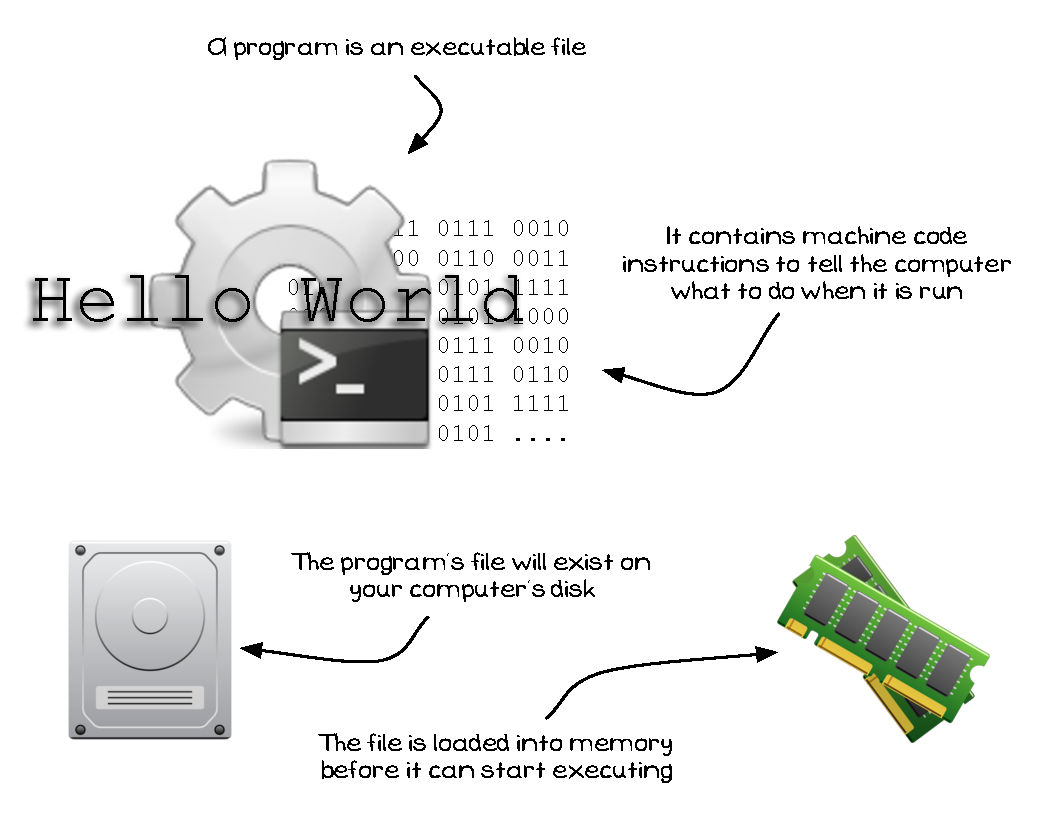
\includegraphics[width=0.9\textwidth]{./topics/programs-and-compilers/diagrams/Program} 
   \caption{A program contains instructions that command the computer to perform a task}
   \label{fig:what-is-a-program}
\end{figure}

\mynote{
\begin{itemize}
  \item You can \textbf{run} programs, which gets the computer to follow the instructions found within the program's file.
  \item To run, the program's instructions must first be loaded into memory.
  \item Once in memory, the computer starts running the instructions one after the other.
  \item When the last instruction is completed the program ends.
  \item There are several different ways to run a program:
  \begin{itemize}
    \item You can \emph{double-click} the program in a file browser.
    \item On tablets and app-phones you can \emph{tap} the program's icon.
    \item Advanced uses can enter \emph{text commands} in the Terminal to start programs.
  \end{itemize}
\end{itemize}
}

\clearpage
\subsubsection{What happens when a program runs?} % (fold)
\label{ssub:what_happens_when_a_program_runs_}

When you run a program, regardless of how it is started, the Operating System loads it from disk into memory and then starts it running. It is important that the file you try to run is a program. These are \emph{special} files that contain instructions the computer can understand.

\begin{figure}[h]
   \centering
   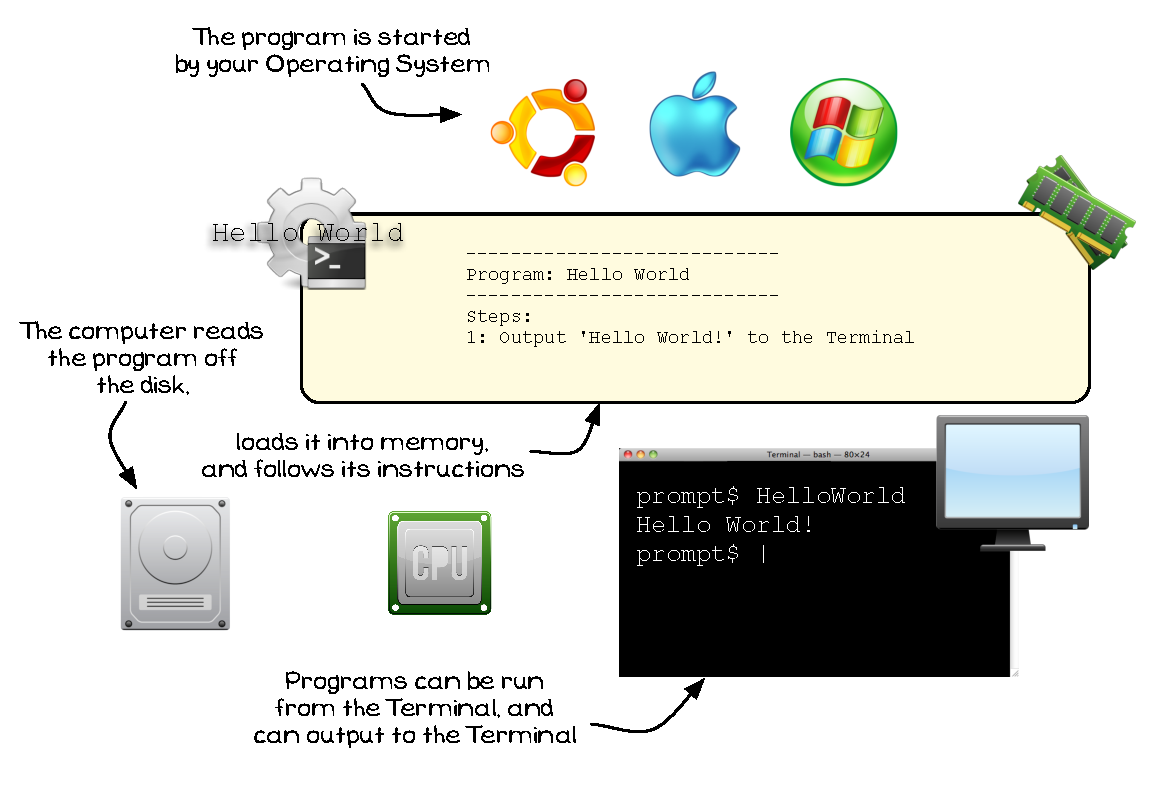
\includegraphics[width=0.9\textwidth]{./topics/programs-and-compilers/diagrams/ProgramExe} 
   \caption{Programs are loaded from disk into memory, then run}
   \label{fig:what-is-a-program-exe}
\end{figure}

\mynote{
\begin{itemize}
  \item Your Operating System is a piece of software that is responsible for managing your computer's hardware.
  \item One of the Operating System's responsible is to start programs.
  \item The \nameref{sub:terminal} can be used to start programs.
  \item Programs can also output to the Terminal.
  \item A Program must contain instructions that the computer can understand.
\end{itemize}
}

% subsubsection what_happens_when_a_program_runs_ (end)

% subsection what_is_a_program_ (end)
\clearpage
\subsection{Machine Code} % (fold)
\label{sub:machine_code}

\emph{What instructions do Computers understand?}

Computers do not really \emph{understand} anything, computers are \textbf{unintelligent}. They are a machine that respond in a set way to a given number of instructions. The instructions that a computer uses is called its {\em instruction set} and contain instructions to perform basic mathematic operations, loading and storing data in memory, comparing numeric values, and moving to the new instruction elsewhere in the program. These very simple actions are performed very quickly, and can be use to create everything you have ever seen a computer do.

The computers instructions can be seen as binary numbers, numbers made from 0's and 1's. These values are like switches that are either off (0) or on (1). Setting these \emph{switches} to different sequences will cause the computer to perform different actions. For example, the \emph{switch} combination \texttt{0000 0011}, may cause the computer to add two numbers together. Any time you want the computer to perform this task you set the switches to that combination. These binary instructions are called \textbf{machine code}.

\begin{figure}[h]
   \centering
   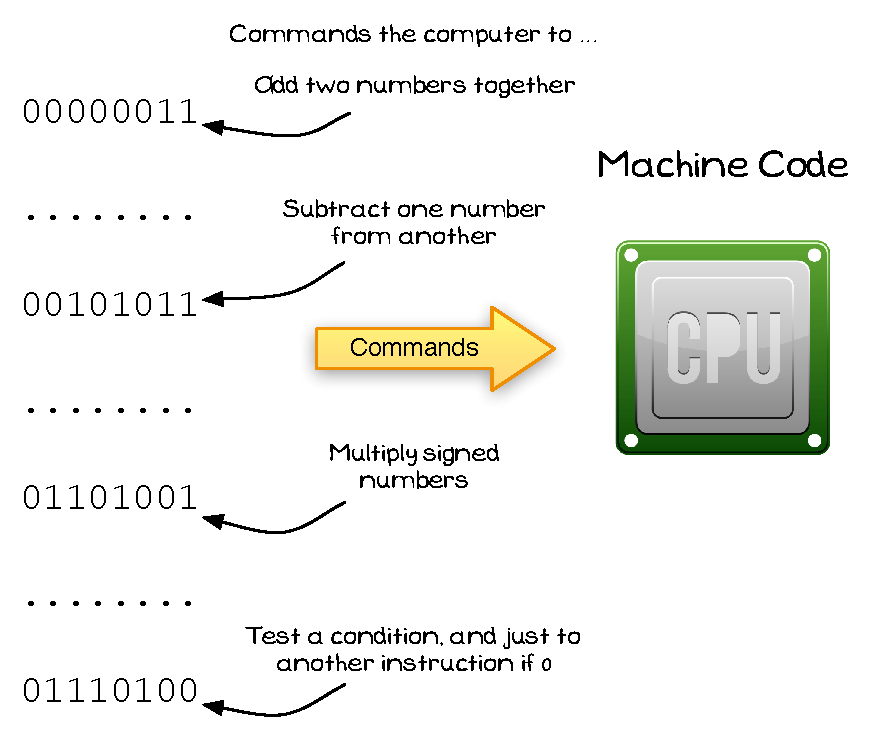
\includegraphics[width=0.8\textwidth]{./topics/programs-and-compilers/diagrams/MachineCode} 
   \caption{The computer responds to machine code instructions}
   \label{fig:machine-code}
\end{figure}

\mynote{
\begin{itemize}
  \item The \textbf{CPU}, Central Processing Unit, is the workhorse of the computer. It executes the program's instructions.
  \item The instructions a CPU uses is called its \textbf{Instruction Set}, and different CPUs have different instruction sets.
  \item Some common instruction sets: ARM (used in iPhones and iPads), x86-64 (used in desktops), and PowerPC (used in the XBox360 and Playstation 3). 
\end{itemize}
}

\clearpage

\subsubsection{Programming in Machine Code} % (fold)
\label{ssub:programming_in_machine_code}

Listing \ref{lst:machine code} shows a chunk of the machine code for a small program. These 1s and 0s are the codes used to instruct the computer when this program is executed. Programs can be written directly in machine code, but this is a time consuming task. This is further complicated by the fact that machine code is unique to each kind of CPU. This means that programming at this level is entirely dependent on the kind of processor that you are targeting.

\begin{lstlisting}[caption={128 bits from the 106,752 bits of Machine Code from a small program.},label={lst:machine code}]
...
0110 0111 0111 0010 0000 0000 0110 0011 0100 1110 0101 1111 0100 0001 0101 1000
0110 0111 0111 0010 0000 0000 0111 0110 0101 1111 0101 1111 0110 1001 0101 1111
...
\end{lstlisting}

No one wants to have to work at this level of details, and fortunately you do not need to. Software developers have created tools to help them create programs without having to think about these low level details. These tools make it possible to work at a \textbf{higher level of abstraction}. They take the code you write, and do the hard work of converting that to the machine code of the computer you want to run it on.

\mynote{
\begin{itemize}
  \item You can look at the machine code of any program on your computer. You just need the right tools.
  \item If you open the program's executable file in a text editor it will look very strange, and not at all like a large list of binary values. This is because the text editor displays one character for every byte (or two bytes depending on the file) from the file.
  \item A \textbf{Hex Editor} is a program that is useful for examining binary data. It shows you one character for every four bits in the file.
\end{itemize}
}

\begin{table}[h]
  \ttfamily
  \centering
\begin{tabular}{|c|c||c|c||c|c||c|c|}
  \hline
  Binary & Hex & Binary & Hex & Binary & Hex & Binary & Hex  \\
  \hline
  0000 & \textbf{0} & 0001  & \textbf{1}  & 0010  &  \textbf{2} & 0011 & \textbf{3} \\
  0100 & \textbf{4} & 0101 & \textbf{5} & 0110 & \textbf{6} & 0111 & \textbf{7} \\
  1000 & \textbf{8} & 1001 & \textbf{9} & 1010 & \textbf{A} & 1011 & \textbf{B} \\
  1100 & \textbf{C} & 1101 & \textbf{D} & 1110 & \textbf{E} & 1111 & \textbf{F} \\
  \hline
\end{tabular}
  \caption{Binary to Hexadecimal}
\end{table}

\begin{figure}[h]
   \centering
   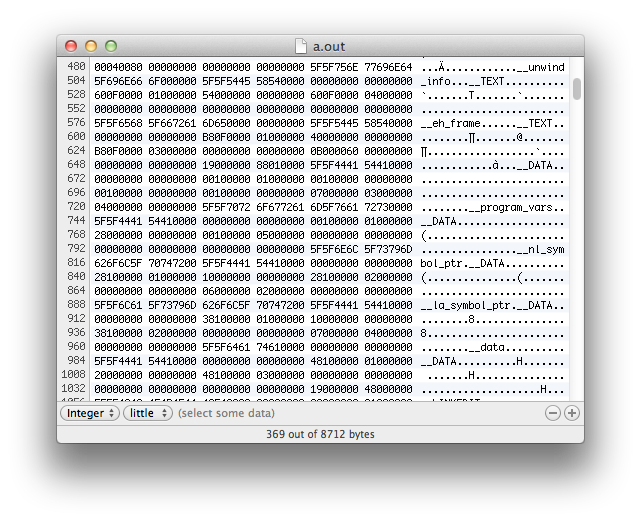
\includegraphics[width=0.55\textwidth]{./topics/programs-and-compilers/images/HexEditor} 
   \caption{A HexEditor allows you to view the machine code of any program}
   \label{fig:hex-editor}
\end{figure}


% subsubsection programming_in_machine_code (end)

% subsection machine_code (end)
\clearpage
\subsection{Assembly} % (fold)
\label{sub:assembly}

The next level of abstraction up from machine code is called \textbf{Assembly}, or \textbf{Assembler Code}. Here the numeric machine code instructions are given symbolic names that are, to some degree, more understandable for humans. The code \texttt{0000 0011} may be given the symbolic name \texttt{add}, for example.

Programs written in this language cannot be executed directly by the computer, it isn't machine code. Assembler code is converted to machine code by a program called an \textbf{Assembler}. This program reads the instructions from the assembler code and outputs machine code. So, for example, anywhere it encounters \texttt{add} in the code it can output \texttt{0000 0011}.

\begin{figure}[h]
   \centering
   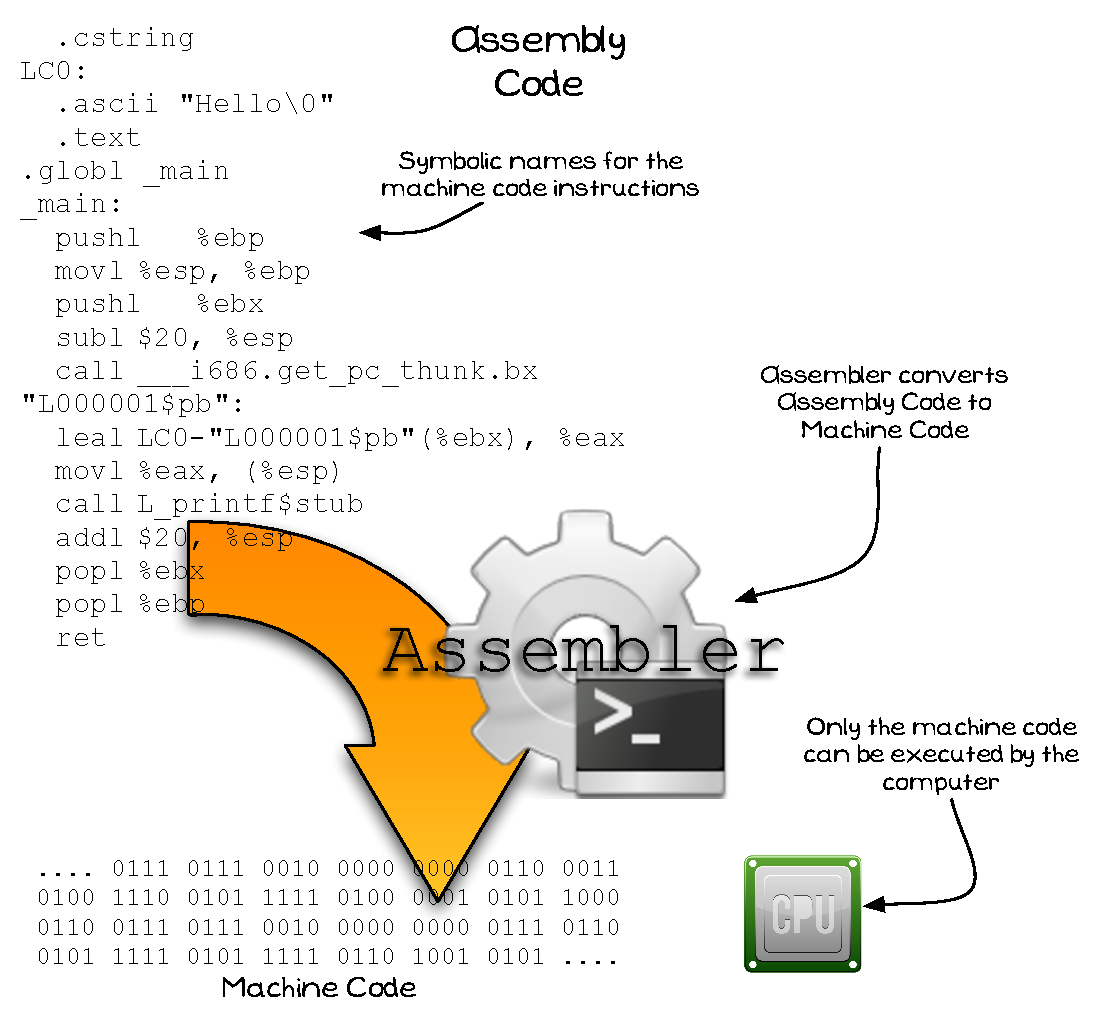
\includegraphics[width=0.8\textwidth]{./topics/programs-and-compilers/diagrams/Assembly} 
   \caption{The computer responds to machine code instructions}
   \label{fig:assembly}
\end{figure}

\mynote{
\begin{itemize}
  \item As with \nameref{sub:machine_code}, Assembly is liked to individual CPUs.
  \item Assembly is very close to Machine Code, its machine code with symbolic names for the instructions.
\end{itemize}
}

\clearpage
\subsubsection{Programming in Assembly} % (fold)
\label{ssub:programming_in_assembly}

The code in Listing \vref{asmcode} shows an example of some assembler code. This is the assembler code that was used to generate the machine code from Listing \ref{lst:machine code}. The machine code was 13,344 bytes in size, where the same program in assembler code is only 658 bytes. The assembler reads these 658 bytes, combines it with instructions from program libraries, and outputs machine code. 
\lstset{language=[x86masm]{assembler}}

\begin{lstlisting}[caption={Assembler Sample},label={asmcode}]
  .cstring
LC0:
  .ascii "Hello\0"
  .text
.globl _main
_main:
  pushl	%ebp
  movl	%esp, %ebp
  pushl	%ebx
  subl	$20, %esp
  call	___i686.get_pc_thunk.bx 
"L000001$pb":
  leal	LC0-"L000001$pb"(%ebx), %eax
  movl	%eax, (%esp)
  call	L_write_line$stub
  addl	$20, %esp
  popl	%ebx
  popl	%ebp
  ret
\end{lstlisting}

From a programmer's perspective, assembler code is much easier to work with than machine code, though there are still issues with the use of assembler code. Firstly Assembly is bound to the instruction set of the CPU that you are targeting, meaning that if you want to support other kinds of CPU you will need to rewrite the program. The other main issue with assembler code is that while it is more understandable, you are still working with the primitive instructions of the CPU. Working at this level takes considerable effort to write even simple programs.

Assembly languages were first developed in the 1950s, and were known as a \textbf{Second Generation}\footnote{First Generation being Machine Code.} programming languages. This step forward did make programming easier, but the tools have advanced since then and now we can work at an even higher level of abstraction.

% subsubsection programming_in_assembly (end)

% subsection assembly (end)
\clearpage
\subsection{Source Code and the Compiler} % (fold)
\label{sub:source_code_and_the_compiler}

The next step in programming language evolution moved from machine level instructions to something more human readable. These languages, known as \textbf{Third Generation Languages}, use move advanced programs than assemblers to convert their instructions into machine code. Programs written in these languages have their code converted to machine code by a \textbf{compiler}.

A \textbf{Compiler} is a program that converts \textbf{Source Code} into machine code that is saved into an executable file called a \emph{Program}. The program can then be executed independent of the compiler and the source code.

Internally, a compiler will perform a number of steps, as shown in \fref{fig:compiler}.

\begin{enumerate}
  \item \textbf{Preprocessing}: The code is read from your source code files. This may involve some processing of the text itself, which includes things like ignoring any comments in the code.
  \item \textbf{Compiling}: The code is then converted into assembly instructions, and an assembly program is output.
  \item \textbf{Assembling}: The assembly version of the program is converted into machine code, and stored in \textbf{object files}.
  \item \textbf{Linking}: In the final step the compiler uses a \textbf{Linker} to join together the machine code from your program, with other machine code you have used from the programming libraries. This then outputs an executable program.
\end{enumerate}

\begin{figure}[h]
   \centering
   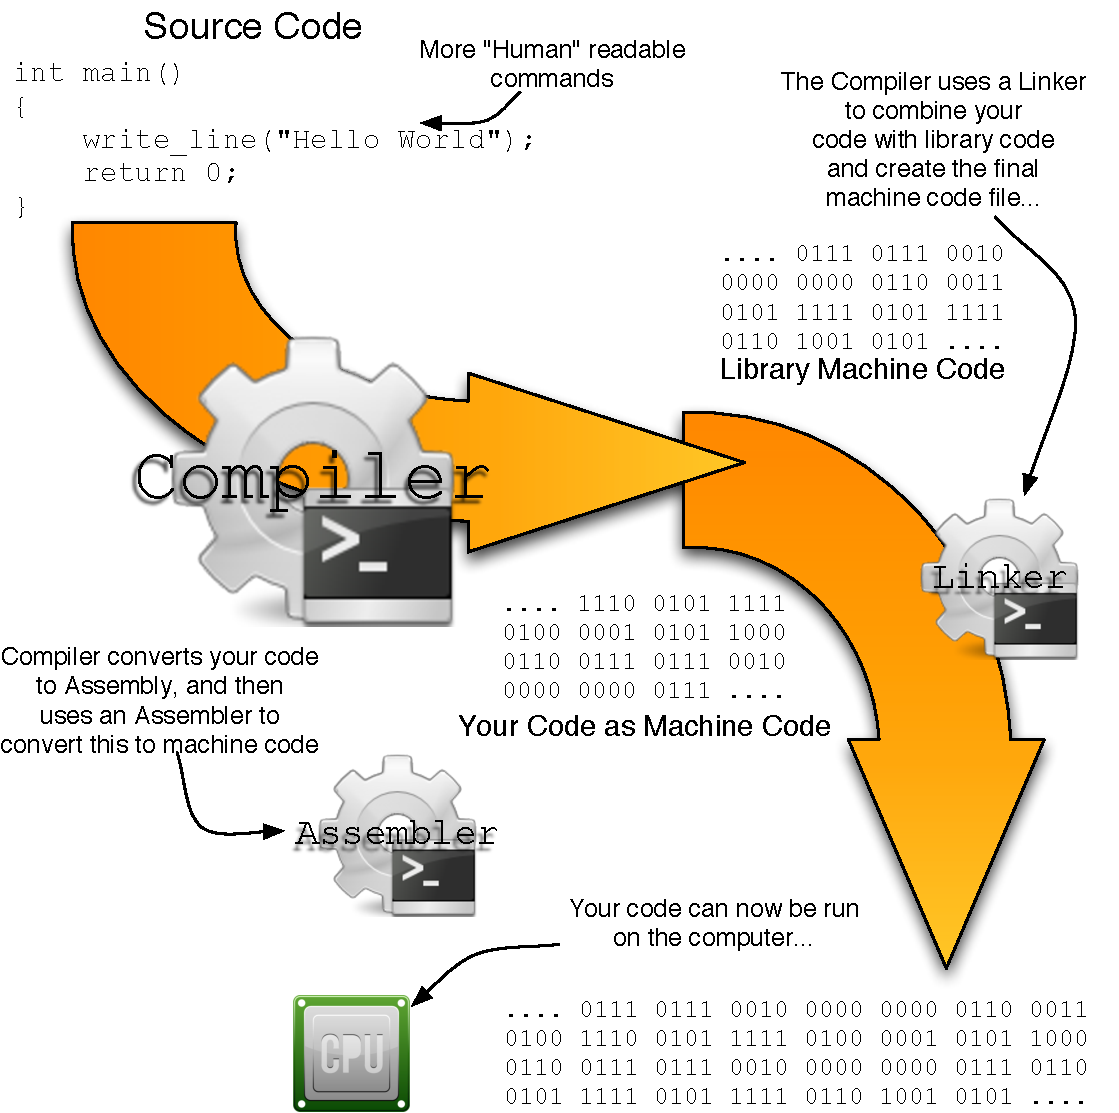
\includegraphics[width=0.8\textwidth]{./topics/programs-and-compilers/diagrams/Compiler} 
   \caption{Compilers turn Source Code into Machine Code}
   \label{fig:compiler}
\end{figure}

\clearpage
\subsubsection{Programming with a Third Generation Language} % (fold)
\label{ssub:programming_with_a_third_generation_language}

\lref{lst:hello-world-c-1} and \lref{lst:hello-world-pas-1} show two examples of source code. This code describes a small program that can be used to output a message to the \nameref{sub:terminal}.

\begin{multicols}{2}
  \ccode{lst:hello-world-c-1}{Example C code}{code/c/program-creation/hello-world.c}
  \columnbreak
  \pascode{lst:hello-world-pas-1}{Example Pascal code}{./topics/program-creation/pascal/HelloWorld.pas}
\end{multicols}

The code shown in \lref{lst:hello-world-c-1} shows the code for the C program that was used to generate the assembler code, and machine code shown in the previous code listings. This code must be converted by the C compiler into machine code before it can be run. It is interesting to note the size of the C file: it is only 50 bytes! The compiler converts this 50 bytes into the 13,344 bytes of machine code. 

\lref{lst:hello-world-pas-1} shows the same program written in the Pascal programming language. Like its equivalent C code, this must be compiled to create a program you can run.

Programs written in a third generation programming language are much easier to understand than their assembler or machine code counterparts. It is also possible that this code can be compiled to run on different types of CPU, making it more portable. Most modern programming languages are third generation programming languages.


The code that a programmer writes in these languages is called \textbf{Source Code}. Typically source code is saved into a text file with a file extension that helps identify the language it is written in. For example, programs written in the C language are saved into files with a {\tt .c} file extension whereas Pascal programs are saved into files with a {\tt .pas} extension.

\mynote{
\begin{itemize}
  \item There are may different Third Generation Languages, including both C and Pascal.
  \item Each language has its own compiler that understands that language's code.
  \item The C compiler we will use is called \textbf{gcc} - this stands for \textbf{GNU C Compiler}.
  \item The Pascal compiler we will use is called \textbf{fpc} - this stands for \textbf{Free Pascal Compiler}.
\end{itemize}
}



% subsubsection programming_with_a_third_generation_language (end)

% subsection source_code_and_the_compiler (end)
% \clearpage
\subsection{Challenges and Rewards} % (fold)
\label{sub:challenges_and_rewards}

% subsection challenges_and_rewards (end)

Programming in a third generation language, like C++ and Pascal, requires you to master several different things, as shown in the following list. The following chapters will work on building your knowledge and skills in each of these aspects.

\begin{enumerate}
  \item What is it that you want the program to do? Writing a program is like writing instructions for someone to carry out. If you do not know how to perform the task yourself you will not be able to tell someone else how to perform the task.
  \item You need to understand what the computer is capable of doing. Computers are unintelligent, so writing a program is more challenging than giving instructions to a person as the computer cannot interpret what you mean and will follow your instructions to the letter, regardless of the effect. The capabilities of the computer limit the flexibility you have for expressing your solution.
  \item The language you choose to develop with also limits how you express your solution. You need to understand the artefacts that you can create, how these artefacts are written in source code, and how these are executed by the computer.
  \item Finally you need to understand how to locate and correct issues with your programs. This includes responding to syntax errors reported to you by the compiler, as well being able to locate errors where the program does not operate the way you intended. 
\end{enumerate}

\emph{With all of these challenges, what appeal does software development have?}

There is nothing better than seeing a program you created running on a computer. You have brought the machine to life, getting it to perform a task the way you want it performed. Once you get a program working it can become easy to get hooked and working on new features and functions becomes a real joy. The greater the challenge the program offers, the greater your sense of achievement when you see the working product in operation.

% subsection compiling_code (end)
\clearpage
\subsection{Terminal} % (fold)
\label{sub:terminal}

Once you have written some source code, you need to be able to compile it. This means, you need to run the \textbf{compiler}, and give it your source code files to compile. The best way to do this when you really want to learn about programming, is to run the compiler directly yourself. To do this you needed to use a \textbf{Terminal} program.

The Terminal is a program that gives you command line access to the computer. With command line access you can enter text commands to start programs. These programs can output details back to the Terminal for you to read, and interactive programs can also read input from you via this same Terminal.

\begin{figure}[h]
   \centering
   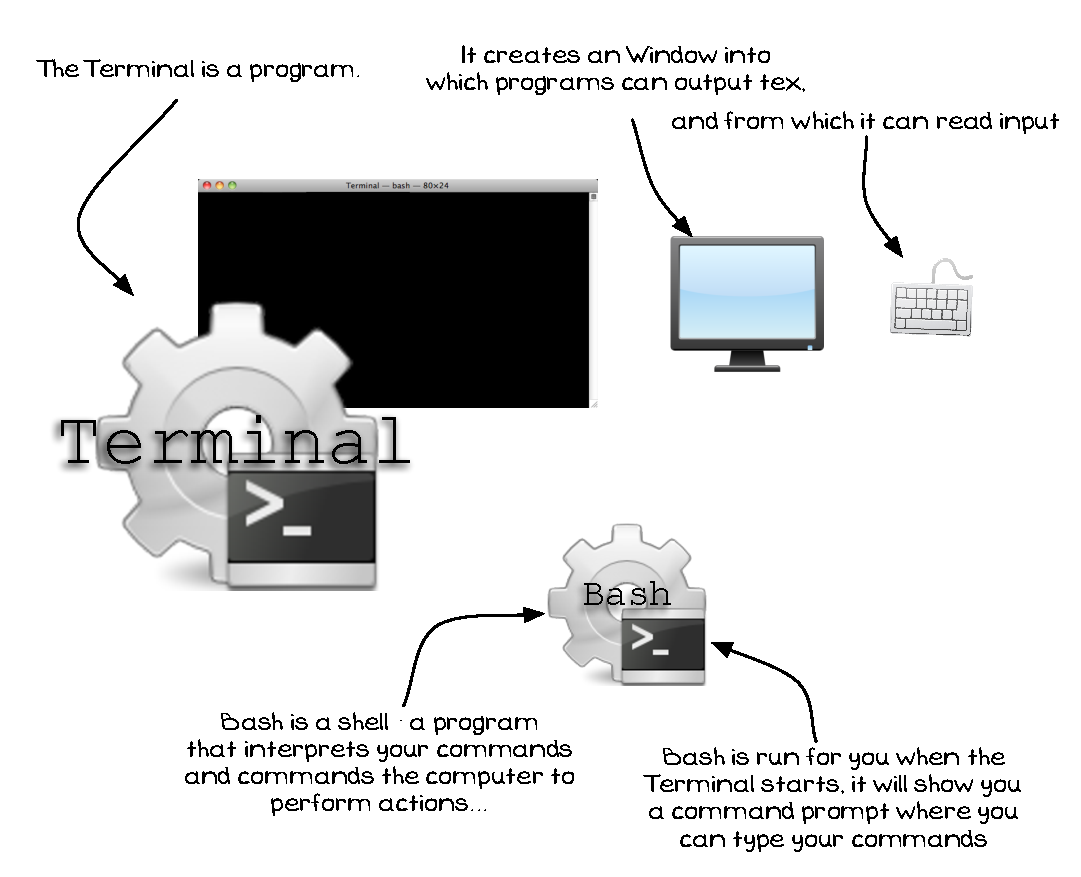
\includegraphics[width=0.8\textwidth]{./topics/programs-and-compilers/diagrams/Terminal} 
   \caption{The Terminal program gives you command line access to your computer}
   \label{fig:terminal}
\end{figure}

\mynote{
\begin{itemize}
  \item On Ubuntu \textbf{Linux} you can find the Terminal in the \emph{Accessories} folder within \emph{Applications}. See Figure \ref{fig:program-creation-ubuntu-terminal}.
  \item On \textbf{MacOS} you can find the Terminal in the \emph{Utilities} folder within \emph{Applications}. See Figure \ref{fig:program-creation-macos-terminal}.
  \item On \textbf{Windows} you will need to download and install \emph{MSys2}. The \emph{MSys2 Shell} is the equivalent of Terminal on the other operating systems. The details for how to install this are in the SplashKit installation guides.

  \item The Terminal is also be called the \textbf{console} or \textbf{command prompt}.
\end{itemize}
}

\clearpage
\subsubsection{The Shell} % (fold)
\label{ssub:the_shell}

The \textbf{Terminal} program itself just provides a text environment, allowing text input and output. Within this environment a \textbf{Shell} program is run to interpret your commands. This is an interactive program that will display a prompt to you, at which you enter your commands.

There are a number of different Shell programs, each of which has its own set of instructions. The Shell we are going to use in this book is called \textbf{Bash}. This shell program is available on Linux, Mac OS, and Windows. As a Unix shell it is native for Linux and Mac OS, and with Windows you can install \textbf{MSys2} to use these commands.

\begin{figure}[h]
   \centering
   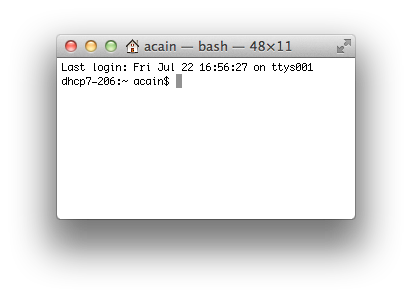
\includegraphics[width=0.6\textwidth]{./topics/programs-and-compilers/images/Bash} 
   \caption{The Terminal running Bash}
   \label{fig:bash}
\end{figure}

A shell program is very simple. It provides a text prompt at which you can enter commands. The Shell then reads the text you entered, and performs an action based on the text you entered. You can use the Shell to perform operations like copying and deleting files, and starting programs.

\mynote{
\begin{itemize}
  \item The name `Shell' came from idea that this was the outermost \emph{shell} of the computer, the interface between the user and the computer's internals.
  \item Bash stands for `\emph{Bourne-again shell}', as Bash is a replacement for the \emph{Bourne} shell.
  \item It will take some time to get used to using Bash, but the more you learn about it the more useful it will become.
\end{itemize}
}

% subsubsection the_shell (end)
\clearpage
\subsubsection{Using Bash} % (fold)
\label{ssub:bash}

To get started using Terminal you will need to know some Bash commands, see \tref{tbl:bash-commands}.

\begin{table}[h]
  \centering
  \begin{tabular}{|l|l|p{5cm}|}
    \hline
    \textbf{Action} & \textbf{Command} & \textbf{Description} \\
    \hline
    Change Directory & \texttt{cd} & Moves the shell to a different working directory. \\
    \hline
    Print Working Directory & \texttt{pwd} & Outputs the current working directory.\\
    \hline
    List Files & \texttt{ls} & Outputs a list of files.\\
    \hline
    Copy File(s) & \texttt{cp} & Copies files from one location to another.\\
    \hline
    Move File(s) & \texttt{mv} & Moves files from one location to another.\\
    \hline
    Delete File(s) & \texttt{rm} & Removes files from the computer. There is no recycle bin with this, so take care!\\
    \hline
    Create a Directory & \texttt{mkdir} & Makes a new directory. \\
    \hline
  \end{tabular}
  \caption{Some bash commands to get you started}
  \label{tbl:bash-commands}
\end{table}

To get started with Bash, you need to understand a little bit about the \textbf{file system}. Each operating system needs a way of storing its files, and there are going to be lots of files stored on a computer. This means that it would be cumbersome to try and keep these all in one place. Instead, the Operating System places files in \textbf{directories} (also known as \emph{Folders}). A directory can contain files, and other directories. 

When you are working in Bash, you will have a \textbf{working directory}. This is the directory where Bash will start searching for the files you are interacting with. To start working with the compiler you will need to be able to use the \textbf{change directory} command to move to the directory that contains your source code files.

With the \textbf{Change Directory} command you tell Bash which directory you want to move into, with the different parts of this path being separated by forward slashes (/). Example commands to move to your Documents directory are shown in \tref{tbl:dirs}, with screenshots for Linux in \fref{fig:linux-files}, Mac OS in \fref{fig:mac-files}, and Windows in \fref{fig:win-files}.

\begin{table}[h]
  \centering
  \begin{tabular}{|l|l|}
  \hline
  \textbf{Operating System} & \textbf{CD Command}  \\
  \hline
  \emph{Linux} & \texttt{cd /home/\emph{uname}/Documents} \\
  or & \texttt{cd $\sim$/Documents} \\
  \hline
  \emph{Mac OS} & \texttt{cd /Users/\emph{uname}/Documents} \\
  or & \texttt{cd $\sim$/Documents} \\
  \hline
  \emph{Windows} & \texttt{cd /c/Users/\emph{uname}/Documents} \\
  \hline
\end{tabular}
  \caption{CD command to move into your documents directory on various Operating Systems. In these examples \texttt{\emph{uname}} should be replaced by your user name. The examples in \fref{fig:linux-files}, \fref{fig:mac-files}, and \fref{fig:win-files} are for the user \texttt{acain}.}
  \label{tbl:dirs}
\end{table}

\mynote{
\begin{itemize}
  \item You can find many resources on using Bash on the web, a fairly extensive overview of these commands can be found at \url{https://dev.to/awwsmm/101-bash-commands-and-tips-for-beginners-to-experts-30je}.
  \item After you run the \texttt{cd} command, you can check which directory you are in using the \textbf{pwd} command. To do this just type \texttt{pwd} and press enter.
  \item Once you get used to the \texttt{cd} command you can start exploring the other commands.
\end{itemize}
}

\begin{figure}[p]
   \centering
   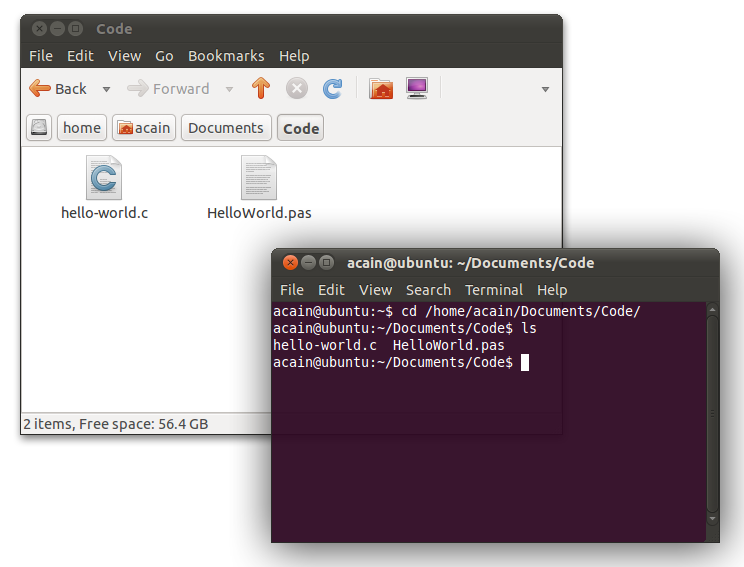
\includegraphics[width=0.9\textwidth]{./topics/programs-and-compilers/images/LinuxFiles} 
   \caption{Changing directories in Linux (Ubuntu)}
   \label{fig:linux-files}
\end{figure}

\begin{figure}[p]
   \centering
   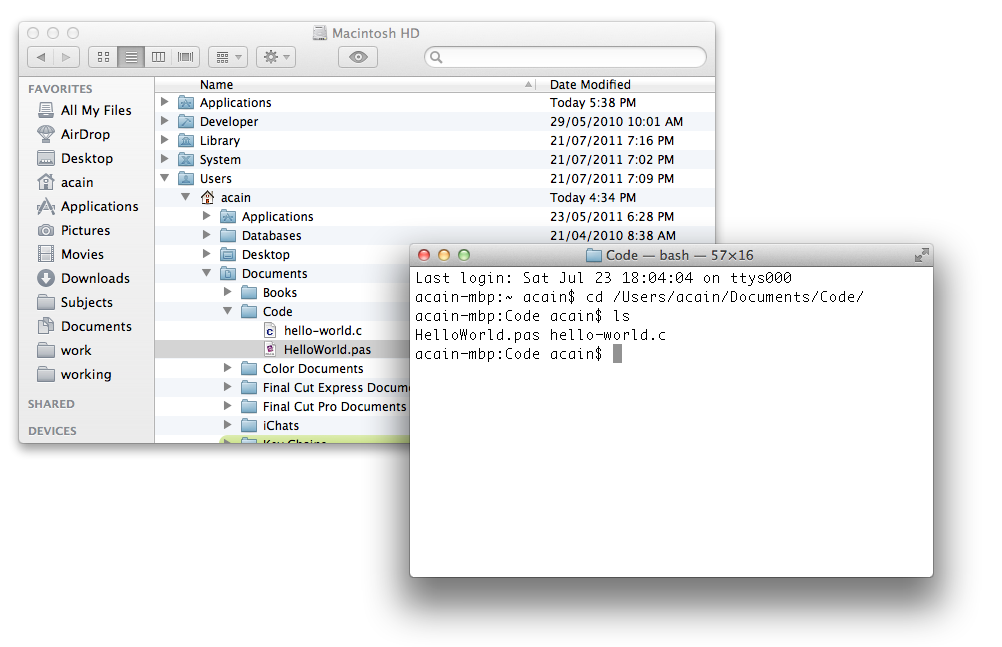
\includegraphics[width=0.9\textwidth]{./topics/programs-and-compilers/images/MacFiles} 
   \caption{Changing directories in MacOS}
   \label{fig:mac-files}
\end{figure}


\begin{figure}[p]
   \centering
   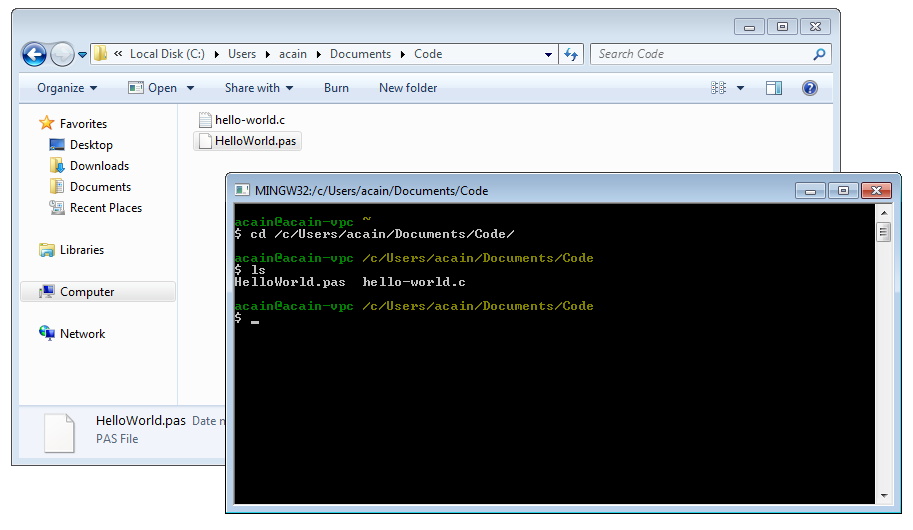
\includegraphics[width=\textwidth]{./topics/programs-and-compilers/images/WindowsFiles} 
   \caption{Changing directories in Windows}
   \label{fig:win-files}
\end{figure}



% subsubsection bash (end)

% subsection terminal (end)
\clearpage
\subsection{The First Program: Hello World} % (fold)
\label{sub:hello world}

There is one very special program that all developers create. This is the first program a software developer creates when they start using a new language, or technology. It is the famous \textbf{Hello World}!

This is a very simple program, it runs and outputs the text `Hello World' to the Terminal. So, why is this the first program? It makes sure that everything is set up correctly. If `Hello World' does not work, then there is something wrong with your setup you need to check.

Listings \ref{lst:hello-world-c} and \ref{lst:hello-world-pas} show the code for the `Hello World' program written with the C++ and Pascal programming languages. Both programs result in the same output when run: they write the text `Hello World!' to the Terminal. They both use the same basic programming structures, and they both go about performing the task in the same way. At this stage, however, they are both just fancy text. What we need to do is use a special tool to convert these into \emph{programs}, we need to \textbf{compile} them.

\csection
{
\ccode{lst:hello-world-c}{Hello World code in C++.}{code/c/program-creation/hello-world.c}
}

\passection{
 \pascode{lst:hello-world-pas}{Hello World code in Pascal.}{./topics/program-creation/pascal/HelloWorld.pas}
}

\mynote{
\begin{itemize}
  \item This source code needs to be written into a \textbf{text file}.
  \item C++ source code usually has a \textbf{.cpp} file extension. For example, \textbf{hello-world.cpp}.
  \item Pascal source code usually has a \textbf{.pas} file extension. For example \textbf{HelloWorld.pas}.
  \item It is a good idea to create a directory (folder) under which you will place your code. Within this directory you can create other directories for individual projects, or for the code related to the chapters in this book.
\end{itemize}
}

% section hello world (end)

\clearpage
\subsection{Making the Hello World Program} % (fold)
\label{sub:compiling_code}

\lref{lst:hello-world-c} and \lref{lst:hello-world-pas} show the source code for the Hello World program. To make this into a program you need to:

\begin{enumerate}
  \item Write the code into a text file.
  \item Save the text file to disk.
  \item Compile it.
\end{enumerate}

Step 1 and 2 can be accomplished with any text editor, but the best ones to use highlight your code. Each programming language has rules that determine how its code must be formatted. This is known as the language's \textbf{syntax}. You can get text editors that understand these rules, and highlight your code as you type. This is called \textbf{syntax highlighting}. This highlighting can help you identify any little mistakes you make. \fref{fig:linux-editors} shows the Hello World code in gedit in Linux. \fref{fig:mac-editors} shows the code in TextMate on Mac OS. \fref{fig:windows-editors} shows the code in Notepad++ in Windows.

\begin{figure}[h]
   \centering
   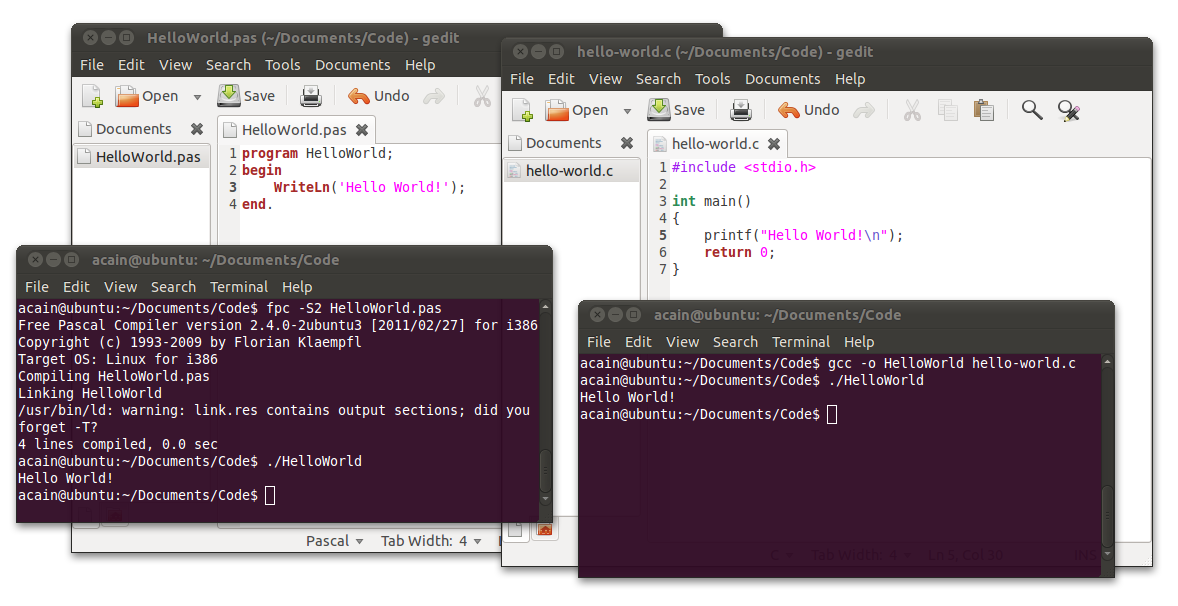
\includegraphics[width=\textwidth]{./topics/programs-and-compilers/images/LinuxEditors} 
   \caption{Editing and Compiling C and Pascal code in Linux}
   \label{fig:linux-editors}
\end{figure}

\begin{figure}[h]
   \centering
   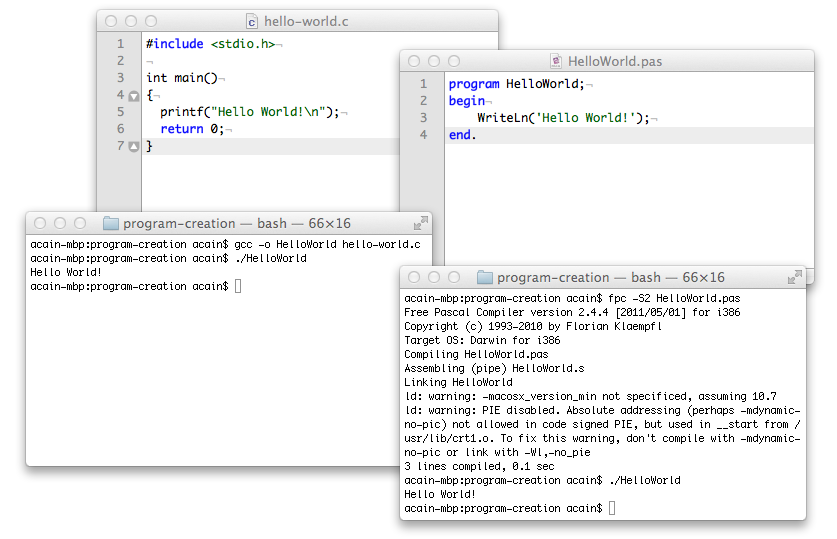
\includegraphics[width=\textwidth]{./topics/programs-and-compilers/images/MacEditors} 
   \caption{Editing and Compiling C and Pascal code in Mac OS}
   \label{fig:mac-editors}
\end{figure}

\begin{figure}[h]
   \centering
   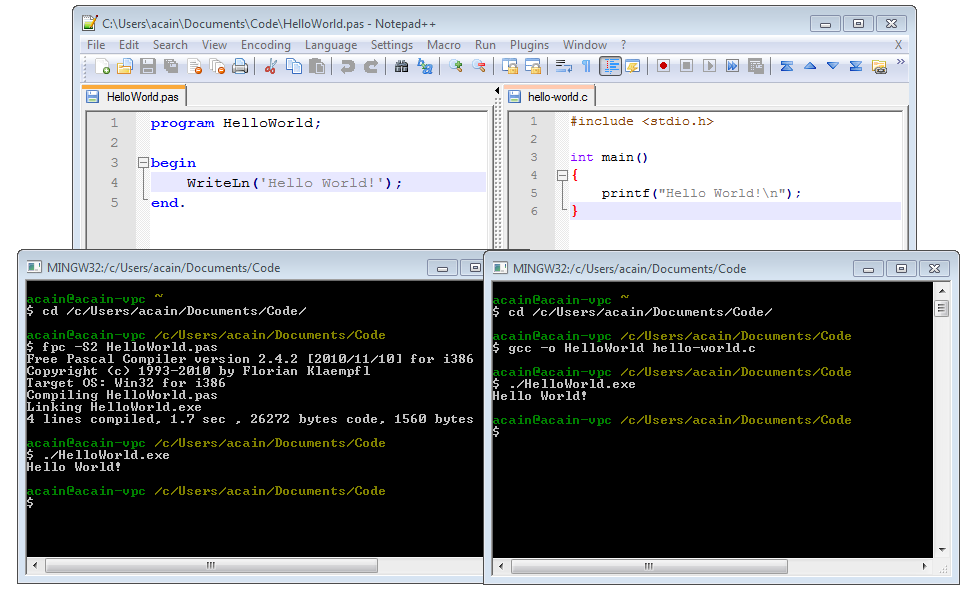
\includegraphics[width=\textwidth]{./topics/programs-and-compilers/images/WindowsEditors} 
   \caption{Editing and Compiling C and Pascal code in Windows}
   \label{fig:windows-editors}
\end{figure}


\mynote{
\begin{itemize}
  \item Syntax highlighting editors include:
  \begin{itemize}
    \item \textbf{gedit} on Linux.
    \item \textbf{TextMate} or \textbf{TextWrangler} on MacOS.
    \item \textbf{Notepad++} or \textbf{Crimson Editor} on Windows.
  \end{itemize}
  \item Take care when you type the code in, even one character out of place may mean the compiler fails to compile your code.
\end{itemize}
}

\clearpage
\subsubsection{Running the Compiler} % (fold)
\label{ssub:running_the_compiler}

When you run the compiler you will pass to it two kinds of information: options, and the file or files you want converted to machine code. The compiler will read the files you pass it and use the language's syntax to determine the tasks you want performed. Once it has built up a model of the program it will the write machine code instructions into a program file. When the compiler finishes you can then run the program file and see the computer perform the tasks coded in the source code.

\csection{
\bashcode{lst:compile-hello-world-c}{Compiling C code.}{code/c/program-creation/compile-hello-world.sh}

There are many different C compilers. The one we will use is the \textbf{gcc} compiler, the \textbf{GNU C Compiler} as shown in Listing \ref{lst:compile-hello-world-c}. When you call the compiler you can use the \emph{-o name} option to tell it the name of the program file to create. In our example this will compile the code in \emph{hello-world.c} and save the machine code into a program called \emph{HelloWorld}.}

\passection{
\bashcode{lst:compile-hello-world-pas}{Compiling Pascal code.}{code/pascal/program-creation/compile-hello-world.sh}

Listing \ref{lst:compile-hello-world-pas} shows the instructions to run the \textbf{fpc} compiler. FPC is the \textbf{Free Pascal Compiler}, which can compile a number of different versions of the Pascal language. The \emph{-S2} option is used to tell FPC to compile using the latest `Free Pascal' version of the language. In our example this will compile the code in \emph{HelloWorld.pas} and save the machine code into a program called \emph{HelloWorld}, which it gets from the name of the Pascal file.}

If the source code you try to compile does not follow all of the rules of the language then the compiler will end with an error message. These errors, called \textbf{syntax errors}, could be as small as missing a semicolon (;), or misspelling a name. When the compiler encounters these issues it does not create the executable program, but instead returns a list showing where it got to before it found an error. You can use these error messages to fix the mistakes, and then run the compiler again to generate your program.


% subsubsection running_the_compiler (end)
% section the_compiler (end)

\clearpage
\subsection{Programming Jargon and Concept Taxonomy} % (fold)
\label{sub:concept_taxonomy}

Programming has a lot of its own jargon. As you learn to develop software it is also important that you start to learn this \emph{special language} that software developers use to discuss their programs. You will find that this terminology is used in many places. It is used in programming texts, in discussions between developers, in discussion boards, blogs, anywhere that developers are discussing software development. Having a clear understanding of this terminology will help you make the most of these resources.

The concepts in this book are closely linked to this programming terminology. To help you understand each concept, we have classified them using one of the following categories:

\begin{itemize}
  \item \textbf{Artefact}: An artefact is something that you can create in your code.
  \item \textbf{Action}: Actions are things that you can \emph{command} the computer to do.
  \item \textbf{Term}: These are general terms, used to describe some aspect.
\end{itemize}

When you are reading about the different concepts in this book you can use these classifications to help you think about how you may use the knowledge you are gaining.

\subsubsection{Artefacts} % (fold)
\label{ssub:artefacts}

Artefacts are things that you create in your code. Programming is a very \emph{abstract} activity, you spend most of your time working with concepts and ideas. You write text, code, that will create things within the computer when your code is run. 

When you are learning about a new kind of artefact come up with ways of visualising it. It is a \textbf{thing} that you are creating with your code. Try to picture the artefact within your code. These artefacts are the basic building blocks that you have to work with. You need to be very familiar with them, how they work, and what you can do with them.

% subsubsection artefacts (end)

\subsubsection{Actions} % (fold)
\label{ssub:actions}

Actions get the computer to perform a task. Your actions will be coded within the \textbf{artefacts} that you create, and will define how artefacts behave when they are used. The actions themselves are commands that you issue to the computer. They are executed one at a time, and each kind of action gets the computer to carry out certain tasks.

When you are learning a new kind of action you need to see what this action does. To start with you should play with it, test it out, and see if you can understand what it is getting the computer to do. As you progress you need to start thinking about how you can sequence these actions so that the computer performs the tasks you want it to. There are only a very few kinds of actions, so it is by combining them that you can get the computer to do what you want. 

% subsubsection actions (end)

\subsubsection{Terms} % (fold)
\label{ssub:terms}

The remaining terms are words that developers use to explain concepts. These are not things that you create, or actions that you request. These are just words that you need to \emph{know}.

When you are learning a new term you need to try to commit it to memory. Memorise the terms, try to use them in sentences, explain them to others. All of these tasks will help you understand, and remember these terms.

% subsubsection terms (end)

% subsection concept_taxonomy (end)

% section concepts_related_to_building_programs (end)


% subsection source_code (end)

\section{Getting Setup} % (fold)
\label{sec:getting_setup}

To create programs you are going to need a couple of tools.

\begin{itemize}
  \item A \textbf{compiler} to convert your source code into machine code.
  \item A \textbf{text editor} to enter your code into.
  \item A \textbf{shell} to interact with your computer.
\end{itemize}



% section getting_setup (end)

\section{Summary} % (fold)
\label{sec:summary-compilers}

Computers can execute \textbf{machine code}, but this isn't very friendly for people to read or create. \textbf{Assembler code} provided the first layer of abstraction over machine code, giving symbolic names to the machine code instructions. This was a little easier to work with, but still required considerable work to create programs of even simple functionality. Most modern programs are written from \textbf{third generation languages} such as \textbf{C} and \textbf{Pascal}. With these languages the develop writes source code that is converted by a \textbf{compiler} into machine code.

% section summary (end)

% chapter building_programs (end)